\documentclass{cmppgr}

\usepackage[pdftex]{graphicx}
\graphicspath{{images/}}

\title{Sequence alignment implementation}
\name{Edward Sleightholme$^1$}
\institution{
	$^1$Department of Computer Science, University of East Anglia, UK\\
}

\usepackage{textcomp}
\usepackage{siunitx}

\begin{document}
	\maketitle
	
	
	\section{Introduction}
	
	Sequence alignment is a way of moving sequences of RNA,DNA or proteins so that that they are aligned . This is a important feature as if they are similar they may have similar functional and structural properties. I have implemented several methods for aligning sequences and compared how they work and give results.
	
	\section{Basic Needleman and Wunsch algorithm}
	This is the most simple of my models and it is split in to 2 parts.Making a scoring matrix and tracing back along the matrix to get the highest scoring route.
	
	\subsection{Making a scoring matrix}
	
	The scoring matrix is a way of showing how well different parts of 2 sequences match together. 
	
	\begin{enumerate}  
		\item First make a scoring empty matrix the size of the 2 sequences + 1
		
		Sequences 1 ='AADAA'
		
		
		Sequences 2 ='AAAA'
		
		
		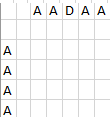
\includegraphics[width=3cm]{firstNormal.png}
		
		\item Assign a gap penalty you want to use. In my example I will be using gap penalty = -8
		
		\item If you have not in the middle of a chain assign these positions zero values to avoid an unnecessary penalty to the alignment
		
		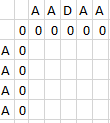
\includegraphics[width=3cm]{secondNormal.png}
		
		\item To fill in rest of table you start in top left empty cell and using algorithm.
		
		g 	= gap penalty 
		
		i,j = position on matrix
		
		s	= the scoring matrix used (For my example is BLOSUM62)
		
		F	= matrix being used
		
		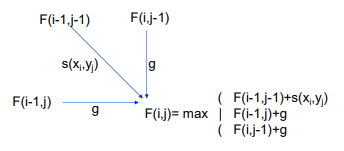
\includegraphics[width=8cm]{fillingInNormal.png}
		
		You can fill in the grids cells with values 
		
		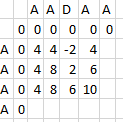
\includegraphics[width=3cm]{thirdNormal.png}

		When you reach the edge of the matrix the algorithm changes so that you stop applying a gap penalty after once you have reached the end of one the sequences.
	
		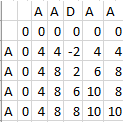
\includegraphics[width=3cm]{forthNormal.png}
		 
		 With that you now have a completed scoring matrix.
		
	\end{enumerate}
	
	\subsection{Trace back}
		Trace back works by starting off at the bottom right corner of the scoring matrix and seeing what possible moves that could be made from that position and then moving to that new position and repeating this process until you reach the top left corner of the matrix. If there are multiple routes that can be taken go though the routes one at a time.
		
		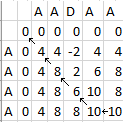
\includegraphics[width=3cm]{traceback.png}
		
		It is better to start from the bottom right of the matrix as there are less chance that you will have to test false paths than if you start at the top left.  
		
		You record the path you take and from that you are able to get a sequence alignment.The score for the alignment is the value in the bottom right hand of the scoring matrix.
	
	
	\section{Local Alignment: The Smith-Waterman Algorithm}
	
	Works in a similar way to Basic Needleman and Wunsch algorithm but focuses on getting a smaller part of a chain that is the most aligned.
	
	It works the same as the Needleman and Wunsch algorithm but the scoring matrix also enables the value 0 at anypoint in the matrix.
	
		g 	= gap penalty 
		
		i,j = position on matrix
		
		s	= the scoring matrix used (For my example is BLOSUM62)
		
		F	= matrix being used
	
	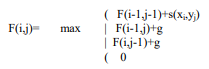
\includegraphics[width=6cm]{localAlginment.png}
	
	
	 The trace back algorithm changes as well as instead of starting at the bottom right corner of the scoring matrix it starts for the point in the matrix with the highest score and the trace back ends when it reaches a value of 0 in the grid
	
	\section{Growing Gap penalty + Opening penalty}
	These two forms of alignment work like Needleman and Wunsch algorithm but they ajust the idea of how gaps should be scored. 
	\subsection{Growing Gap penalty}
	This version of the algorithm works on the idea that the bigger the gap you have in a sequence the greater the gap penalty should get. You can apply this to an linear equation. This method requires you to keep track of how many gaps have happened on each matrix position.
	
	n= length of gap 
	
	g = gap penalty 
		
	y(n)= gap penalty to apply 
	
	\[ y(n) = ng \] 
	
	This causes the algorithm to punish long gaps more and more as they grow.
	
	\subsection{Opening penalty}
	This version of the algorithm works on the idea that starting a gap in a alignment should be avoided adds an additional penalty to starting a gap in the alignment. Gap penalty can be combined with the idea of a growing gap penalty as well to give this equation.
	
	
	g =	the opening gap penalty
	
	
	e =	gap extension penalty 
	
	
	n= length of gap 
	
	y(n)= gap penalty to apply 
	
	\[ |e| < |g| \]
	
	\[y (n) = g + (n − 1) e\]
	
	\section{Displaying a Alignment}
	The program displays alignments as shown below.
	
	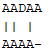
\includegraphics[width=1cm]{alignment.png}
	
	Top line = sequence 1
	
	Middle line = the relationship between the sequences 
	
	Bottom line = sequence 2
	
	 \textbar	= Shows match in alignment

	- = A gap has been made in the alignment 
	
	
\end{document}